\documentclass[11pt]{article}

\usepackage[preprint]{acl}

\usepackage{times}
\usepackage{latexsym}
\usepackage[T1]{fontenc}
\usepackage[utf8]{inputenc}
\usepackage{microtype}
\usepackage{inconsolata}
\usepackage{graphicx}
\usepackage{booktabs}
\usepackage{amsmath}
\usepackage{amssymb}
\usepackage{tikz}
\usetikzlibrary{arrows.meta,positioning}

\title{Sampling the Truth: Decoding Strategies and the\\
       Factuality--Diversity Tradeoff in Small Open LLMs}

\author{Mohummad Nasrallah \\
  213606155 \\
  Tel Aviv University \\
  \texttt{mohummadn@mail.tau.ac.il} \\\And
  Fooad Khalaila \\
  208045898 \\
  Tel Aviv University \\
  \texttt{fooadk@mail.tau.ac.il} \\}

\begin{document}
\maketitle

\begin{abstract}
The decoding algorithm turns one language model into what appear to be
different systems, but factuality and diversity are measured in separate
literatures, on different models, and almost never at a matched inference
budget. We evaluate seven decoding configurations and two diagnostic controls
across three open models spanning 124M to 3B parameters, three seeds and 100
biography prompts --- 8{,}100 generations --- scoring every sentence against
the subject's Wikipedia page with an NLI verifier calibrated against 100 blind
human labels. Beam search is the most factual configuration at every scale and
costs almost all of the diversity, at $3.5\times$ the compute. Under a matched sampler, DoLa's
layer contrast improves on nucleus sampling at all three scales, though at
124M both arms sit at the verifier's floor; its apparent reversal with scale
is an artifact of comparing a greedy-family decoder against a sampling
baseline.
Self-consistency never reaches the support--compute frontier: an oracle
picking the best of its five samples would still lose to beam search at
comparable cost.
At 124M, most apparent factuality is genericity rather than knowledge.
\end{abstract}

\section{Introduction}

A language model defines a distribution over next tokens; the decoding
algorithm decides which token is emitted. The same weights, driven by greedy
search or by nucleus sampling, produce text so different in character that the
two read like separate systems --- one repetitive and conservative, the other
varied and prone to invention.

How that choice should be made is studied in two literatures that do not meet.
Work on degeneration and diversity measures repetition and distinctness, and
largely ignores whether the text is true. Work on factual decoding measures
accuracy on short-answer or multiple-choice benchmarks, and largely ignores
what the method does to the variety of the output. Neither routinely charges a
method for the extra inference compute it consumes, so a technique that samples
five times is compared directly against one that samples once.

We measure both axes together, on the same models, with seed variance, and at a
matched inference budget. The grid is three models (GPT-2 124M, Llama-3.2-1B
and Llama-3.2-3B), seven decoding configurations plus two diagnostic controls,
three seeds and 100 biography prompts: 8{,}100 generations, each scored for
factual support against the subject's Wikipedia page and for diversity,
repetition and fluency. The verifier is not trusted on faith --- it is
validated against 100 blind human labels and its output calibrated by the
measured false-positive rate.

Three findings stand out. Beam search is the most factual configuration at
every scale, and pays for it with almost total loss of diversity and
$3.5\times$ the compute (Figure~\ref{fig:teaser}). DoLa's layer contrast, compared
against nucleus under a matched sampler, improves factual support at all three
scales ($+0.037$, $+0.076$, $+0.079$) at a cost in diversity; the reversal the
unmatched comparison shows belongs to the decoder family, not the contrast.
Self-consistency does not pay for itself --- it lies off the support--compute
frontier at every scale, and the reason is the selector rather than the
samples, since an oracle choosing the best of the five would still lose to
beam search at comparable cost.

The question this work asks is therefore: how does the choice of decoding strategy
--- greedy and beam search, temperature and nucleus sampling, DoLa, and
self-consistency --- affect the tradeoff between factual accuracy and output
diversity in open-ended generation with small open LLMs, and does the picture
change with model scale?

\begin{figure*}[t]
  \centering
  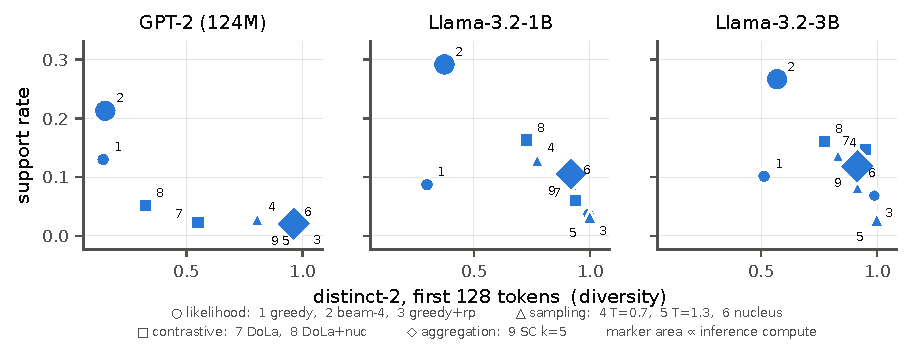
\includegraphics[width=\linewidth]{figures/f1_teaser.pdf}
  \caption{Factuality against diversity for seven decoding configurations and
    two controls, across three model scales, on the 80 test entities. Marker
    area is proportional to inference compute. Beam search occupies the
    high-factuality, low-diversity corner at every scale; every sampling-based
    configuration collapses into a narrow band of near-maximal diversity.}
  \label{fig:teaser}
\end{figure*}

\section{Related Work}

\paragraph{Decoding and degeneration.}
\citet{holtzman2020curious} established that maximising likelihood makes
open-ended text degenerate into repetition, and introduced nucleus sampling as
the remedy. Their evaluation is of diversity and human-judged quality; whether
the more varied text is also more or less \emph{true} is not measured, and the
tradeoff we study is exactly the one their paper leaves open.

\paragraph{Decoding for factuality.}
\citet{li2023contrastive} introduced contrastive decoding, which scores
continuations by the difference between an expert and an amateur model, and
evaluated it on open-ended generation judged for quality rather than factual
accuracy. \citet{chuang2024dola} specialised the idea within a single model:
DoLa contrasts the logits of a late layer against an earlier one, on the
argument that factual knowledge is resolved in the upper layers, and reports
gains on multiple-choice and short-form benchmarks. Factual accuracy in
open-ended generation falls between the two. Also left open are behaviour at
small scale, and whether the repetition penalty DoLa ships with is responsible
for part of the reported effect --- which our \textbf{greedy+rp} control
isolates directly.

\paragraph{Aggregation over samples.}
\citet{wang2023selfconsistency} showed that sampling several chains of thought
and taking the majority answer improves reasoning accuracy. The method requires
a discrete answer to vote on, and is undefined when the output is a paragraph
of free text. Extending it therefore requires replacing equality with
similarity, which is a change to the method rather than an application of it;
we make that change explicit, and test what survives it.

\paragraph{Verifying long-form factuality.}
\citet{min2023factscore} introduced FActScore, which decomposes generated
biographies into atomic facts and verifies each against a reference passage,
and showed that factual precision falls sharply for less prominent entities.
Their protocol is the ancestor of ours and their entity list is the one we
sample from. We deviate in verifying whole sentences rather than
model-decomposed atomic facts, which removes a language model from the
measurement loop at the cost of coarser units. What their evaluation does not
address, and ours does, is how the factual precision of a fixed model changes
with the decoding algorithm applied to it.

\paragraph{Positioning against prior course work.}
A previous project in this course \citep{mark-frenkel} studied self-consistency
for summarisation, validating roughly 117 samples by manual annotation. Our
design differs on four axes: the task is open-ended factual generation;
verification is automatic and therefore applied to 8{,}100 generations rather
than a hundred; the comparison spans the full single-pass decoding space rather
than one aggregation method; and every configuration is priced in inference
compute. Human annotation \emph{calibrates} the automatic verifier rather than
replacing it.

\paragraph{The gap.}
Factuality and diversity are each well studied and almost never studied
together. Where they are measured jointly it is usually on one model, without
seed variance, and without pricing the inference compute a method consumes ---
which flatters exactly those methods that consume the most. No published
comparison holds the model, the prompts, the seeds and the budget fixed while
varying the decoder. That comparison is what this paper supplies.

\section{Method}

\begin{figure*}[t]
  \centering
  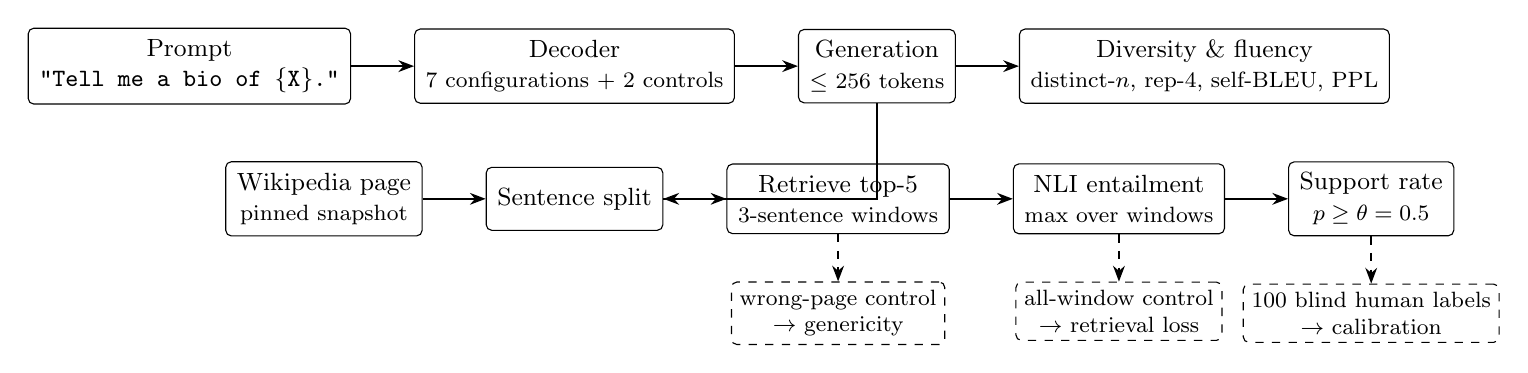
\begin{tikzpicture}[
    box/.style={draw, rounded corners=2pt, align=center, font=\small,
                inner sep=4pt, minimum height=8mm},
    ctrl/.style={draw, dashed, rounded corners=2pt, align=center,
                 font=\footnotesize, inner sep=3pt, minimum height=7mm},
    ar/.style={-{Stealth[length=2mm]}, semithick},
    dar/.style={-{Stealth[length=2mm]}, semithick, dashed}
  ]
  \node[box] (prompt) {Prompt\\\texttt{"Tell me a bio of \{X\}."}};
  \node[box, right=8mm of prompt] (dec)
       {Decoder\\\footnotesize 7 configurations + 2 controls};
  \node[box, right=8mm of dec] (gen) {Generation\\\footnotesize $\leq$ 256 tokens};
  \node[box, right=8mm of gen] (div)
       {Diversity \& fluency\\\footnotesize distinct-$n$, rep-4, self-BLEU, PPL};

  \draw[ar] (prompt) -- (dec);
  \draw[ar] (dec) -- (gen);
  \draw[ar] (gen) -- (div);

  \node[box, below=8mm of dec] (split) {Sentence split};
  \node[box, right=8mm of split] (ret)
       {Retrieve top-5\\\footnotesize 3-sentence windows};
  \node[box, right=8mm of ret] (nli) {NLI entailment\\\footnotesize max over windows};
  \node[box, right=8mm of nli] (sup) {Support rate\\\footnotesize $p \geq \theta = 0.5$};
  \node[box, left=8mm of split] (page) {Wikipedia page\\\footnotesize pinned snapshot};

  \draw[ar] (gen) |- (split);
  \draw[ar] (split) -- (ret);
  \draw[ar] (page) -- (split);
  \draw[ar] (ret) -- (nli);
  \draw[ar] (nli) -- (sup);

  \node[ctrl, below=6mm of ret] (wrong) {wrong-page control\\$\rightarrow$ genericity};
  \node[ctrl, below=6mm of nli] (allw) {all-window control\\$\rightarrow$ retrieval loss};
  \node[ctrl, below=6mm of sup] (hum) {100 blind human labels\\$\rightarrow$ calibration};

  \draw[dar] (ret) -- (wrong);
  \draw[dar] (nli) -- (allw);
  \draw[dar] (sup) -- (hum);
  \end{tikzpicture}
  \caption{The pipeline. One prompt per entity is decoded under each of seven
    configurations and two controls; the generation is scored for diversity and
    fluency directly, and for factuality by splitting it into sentences,
    retrieving evidence windows from the entity's Wikipedia page, and asking an
    NLI model whether each window entails each sentence. Dashed boxes are the
    validity controls: the same claims re-scored against a different entity's
    page, against every window of the correct page, and against 100 blind human
    labels.}
  \label{fig:method}
\end{figure*}

\subsection{Task}

Each system is asked to produce a biography of a named person with the prompt
\texttt{"Tell me a bio of \{entity\}."}, used verbatim from FActScore
\citep{min2023factscore} for comparability. The models are base rather than
instruction-tuned, so the prompt is completed as raw text; a more instructive
prompt would compress the very differences between decoders that this study
measures.

\subsection{Decoding configurations}

We compare seven decoding configurations: greedy search, beam search with four
beams, temperature sampling at $\tau=0.7$ and $\tau=1.3$, nucleus sampling at
$p=0.9$ \citep{holtzman2020curious}, DoLa \citep{chuang2024dola}, and
self-consistency with $k=5$ \citep{wang2023selfconsistency}. Two further
configurations are included as controls rather than as candidate methods.
\textbf{greedy+rp} applies DoLa's repetition penalty to greedy decoding
without the layer contrast, isolating how much of DoLa's behaviour is the
penalty rather than the contrast. \textbf{DoLa+nucleus} runs DoLa on top of
nucleus sampling, so DoLa can be compared against nucleus under an identical
sampler. Every configuration sets \texttt{do\_sample}, \texttt{temperature},
\texttt{top\_p} and \texttt{top\_k} explicitly, because the model families ship
different generation defaults and inherited values would make the arms
non-comparable across models.

Self-consistency requires a modification we state plainly. Majority vote over
answers is undefined for open-ended text: five biographies are never
string-identical, so the vote is vacuous. We replace equality with similarity
and keep the sample with the highest mean cosine similarity to the other four
under a sentence encoder --- the embedding medoid. What we evaluate is
therefore ``sample five, keep the medoid'', not self-consistency as originally
defined. Because a selector can never beat the pool it is given, we also report
the oracle best-of-five bound.

\subsection{Factuality: sentence-level support}

A generation is split into sentences; each sentence becomes a claim to verify
against the entity's Wikipedia page. We retrieve the five most relevant
three-sentence windows of the page using a hybrid of BM25
\citep{robertson2009bm25} and dense retrieval \citep{reimers2019sbert,
song2020mpnet}, and score each window--claim pair with a natural language
inference (NLI) model, which predicts whether a premise entails, contradicts or
is neutral towards a hypothesis. The window is the premise and the claim the
hypothesis; the claim is prefixed with the entity name, because generations say
``She was born\ldots'' where the page says ``Ada Lovelace was born\ldots''. A
claim counts as \emph{supported} if the maximum entailment probability across
its five windows is at least $\theta=0.5$. The maximum is used rather than the
mean because a claim is supported if \emph{any} part of the page supports it.
The \textbf{support rate} of a generation is its fraction of supported
sentences.

We call this support rate and never FActScore: FActScore decomposes text into
atomic facts with a language model, while we verify whole sentences, which is
deterministic and free but collapses mixed-truth sentences onto one label.
Support is not truth; it is agreement with one reference page.

Generations with fewer than two usable sentences are \emph{degenerate}: a single
label would force a score of $0$ or $1$. The verifier flags them and returns no
rate, but every reported number scores them $0.0$, so the prompt set is
identical across arms and each arm is charged for what it failed to produce.

\subsection{Diversity, repetition and fluency}

\textbf{Distinct-$n$} is the ratio of unique to total $n$-grams (1.0 means no
repeats) and \textbf{rep-4} is its complement over 4-grams. \textbf{Self-BLEU}
measures mutual similarity among several generations from one configuration,
and is reported only for stochastic configurations, since a deterministic
decoder returns identical text across seeds and scores 1.0 by construction
rather than by lack of diversity. \textbf{Fluency} is perplexity under a scorer
model disjoint from all three generators. Generation length varies by more than
a factor of two across configurations and distinct-$n$ falls mechanically with
length, so every length-sensitive metric is computed on a fixed 128-token
prefix.

\subsection{Matched inference compute}

Comparing aggregation methods against single-pass decoders without accounting
for cost is unfair to the single-pass methods. Beam search returns one sequence
but decodes $k$ in parallel, and self-consistency draws five samples, so
returned tokens understate their cost by $4\times$ and $5\times$ respectively.
We therefore record
\[
\text{compute} = \text{generated tokens} \times \text{beams} \times \text{samples}
\]
on every record and report every result against it. It counts decoded tokens
rather than arithmetic, so a method that does extra work per step, such as
DoLa's layer contrast, is not charged for it. Wall-clock timing is
CUDA-synchronised.

\subsection{Statistical protocol}

All comparisons are paired over prompts with a bootstrap of 10{,}000 resamples,
with seeds averaged within a prompt. Significance is judged at the three
decimals reported: an interval whose bound prints as $0.000$ is not counted as
excluding zero. Pairing cancels between-entity variance, which dominates:
per-entity rates have $\sigma \approx 0.25$, so an unpaired comparison at
$n=80$ would need gaps of five to seven points. Three seeds are reported
because the proposal promised them, but they are not where statistical power
comes from --- the bootstrap over prompts is. Support rates are macro-averaged
over prompts rather than micro-averaged over sentences, because generation
length varies by configuration and a micro-average would let a length
difference masquerade as a factuality difference.

\section{Experimental Setup}

\subsection{Models}

GPT-2 (124M) \citep{radford2019gpt2}, Llama-3.2-1B and Llama-3.2-3B
\citep{llama3}, all base variants. Alignment lowers output entropy and would
confound scale with instruction tuning; GPT-2 has no instruct variant, so base
keeps all three comparable. All three run in \texttt{float16} on a single
NVIDIA TITAN Xp, the only dtype available at all three scales:
\texttt{bfloat16} is emulated on this card and Llama-3.2-3B exceeds its memory
in \texttt{float32}. Generation uses \texttt{transformers} 5.16.1 and
\texttt{torch} 2.14.0+cu126, both pinned.

DoLa is not available in the core library at this version and runs through a
pinned third-party implementation of the 4.x code
(\texttt{transformers-community/dola}, revision \texttt{af6cdc35}), pre-fetched
so that no run can silently resolve a different revision. What we evaluate is
therefore that implementation rather than the authors' own; this is noted in
Limitations.

\subsection{Entities and splits}

FActScore's published list contains 500 entities, of which 454 resolve in the
pinned Wikipedia snapshot (\texttt{20231101.en}); two independent passes over all
6{,}407{,}814 rows found none of the remaining 46, so the gap is systematic. The missing articles are heavily templated --- major
historical figures and athletes with large statistics tables --- so the pool is
tilted away from the most famous entities.

From the 454 we sample 100 entities stratified into three strata by article
length (Table~\ref{tab:data}), frozen once with a fixed seed and never
regenerated, because choosing entities after seeing results is selection bias.
The snapshot is pinned so that no reference page can contain facts published
after the models were trained.

\textbf{Dev/test discipline.} The 100 entities are split 20 dev / 80 test, fixed
in advance. Every tunable quantity --- the entailment threshold $\theta$,
DoLa's layer selection, the minimum sentence length, and the retrieval-depth
sensitivity sweep --- was chosen on the 20 dev entities, and \textbf{every
comparison between decoding configurations is computed on the 80 test entities
only.} What dev measures is the instrument rather than the arms: the 100 human
labels behind Table~\ref{tab:verifier}, which also set the calibration
constants, and the sweep in Appendix~\ref{app:robustness}. $\theta$ was chosen
to maximise agreement with human labels, never to maximise the gap between
configurations.

\subsection{Generation}

Three seeds (1234, 5678, 9012), fixed before any result was observed.
\texttt{max\_new\_tokens} is 256 for every configuration --- long enough for a
real biography, and identical across arms, on which the fairness of the
comparison depends. The full grid is 3 models $\times$ 9 configurations
$\times$ 3 seeds $\times$ 100 prompts $=$ \textbf{8{,}100 generations}. Cap
rates range from 40\% to 89\% across configurations, which is why every
length-sensitive metric is also computed on a fixed prefix.

\subsection{Verifier}

The NLI model is a DeBERTa-v3-large checkpoint \citep{he2023debertav3}
fine-tuned on MNLI, FEVER, ANLI, LingNLI and WANLI \citep{laurer2024nli}. The
entailment label index is read from the model configuration rather than
hard-coded, and premises are truncated before hypotheses so a claim is never
the text that gets cut. Retrieval uses three-sentence windows
with $m=5$, and the retrieval encoder is \texttt{all-mpnet-base-v2}.

\subsection{Verifier validation and calibration}

The verifier is validated against 100 human labels, drawn stratified by entity
stratum and entailment-probability band so that the sample can estimate both
false positives and false negatives, and presented blind --- without the
model's probability or verdict --- so that the labels cannot drift toward
agreement with the system under test. Labels are entailment-style: a claim is
\emph{supported}, \emph{contradicted}, or \emph{not addressed} by the evidence
shown. The scheme deliberately requires no world knowledge, which makes it
objective but means it cannot separate ``true but absent from the page'' from
``not in the page''; the consequence is stated in Limitations.

The verifier is high-recall and low-precision (Table~\ref{tab:verifier}):
sensitivity $0.947$, false-positive rate $0.041$, balanced accuracy $0.953$.
Balanced accuracy peaks at $\theta=0.55$ ($0.956$), inside noise of the
pre-registered $\theta=0.5$, which is therefore retained without
re-verification. We report support rates both raw, for comparability with
FActScore-style numbers, and calibrated by the Rogan--Gladen correction
\[
T = \frac{R - \mathrm{FPR}}{\mathrm{TPR} - \mathrm{FPR}},
\]
which is prevalence-independent and therefore transfers from the label frame to
each configuration. A configuration whose calibrated interval includes zero is
reported as indistinguishable from zero true support rather than as a small
positive number.

Calibrated intervals resample the 100 labels and the 80 test prompts jointly,
10{,}000 times, so that uncertainty in the verifier's sensitivity and
false-positive rate is carried into the reported rate; values of $T$ below zero,
which arise when a configuration's raw rate falls below the false-positive rate,
are reported as $0.000$.

\subsection{Reproducibility}

All model revisions, library versions, seeds and the entity list are pinned and
committed. Every generation is stored as a record carrying its git commit,
device, dtype and decoding arguments, and every results figure and table in
this paper is generated from those records by a committed script, available at
\url{https://github.com/MohummadN/sampling-the-truth}.

% T1 (dataset statistics) and T2 (main results), generated by scripts/tables.py
\begin{table}[t]
  \centering
  \small
  \begin{tabular}{lrrrrrr}
    \toprule
    \textbf{Stratum} & \textbf{$n$} & \textbf{dev} & \textbf{test} & \textbf{min} & \textbf{med} & \textbf{max} \\
    \midrule
    0 & 34 & 7 & 27 & 20 & 28 & 47 \\
    1 & 33 & 7 & 26 & 31 & 54 & 120 \\
    2 & 33 & 6 & 27 & 61 & 166 & 659 \\
    \midrule
    all & 100 & 20 & 80 & & & \\
    \bottomrule
  \end{tabular}
  \caption{Entity pool. Strata are formed by Wikipedia page length; \textbf{min}, \textbf{med} and \textbf{max} are page sentences. The grid produces 8,100 generations (3 models $\times$ 9 configurations $\times$ 3 seeds $\times$ 100 prompts); all reported results use the test split.}
  \label{tab:data}
\end{table}

\begin{table*}[t]
  \centering
  \small
  \begin{tabular}{ll rrc rr r}
    \toprule
    \textbf{Model} & \textbf{Configuration} & \textbf{Support} & \textbf{Calibrated} & \textbf{95\% CI} & \textbf{Distinct-2} & \textbf{Rep-4} & \textbf{Compute} \\
    \midrule
    GPT-2 (124M) & beam-4 & 0.213 & 0.189 & [0.090, 0.294] & 0.149 & 0.827 & 3.55$\times$ \\
     & greedy & 0.130 & 0.098 & [0.017, 0.179] & 0.140 & 0.833 & 1.00$\times$ \\
     & DoLa+nuc & 0.052 & 0.012$^{\dagger}$ & [0.000, 0.043] & 0.322 & 0.605 & 0.99$\times$ \\
     & T=0.7 & 0.028 & 0.000$^{\dagger}$ & [0.000, 0.011] & 0.805 & 0.085 & 0.97$\times$ \\
     & DoLa & 0.023 & 0.000$^{\dagger}$ & [0.000, 0.008] & 0.550 & 0.346 & 0.98$\times$ \\
     & greedy+rp & 0.022 & 0.000$^{\dagger}$ & [0.000, 0.009] & 1.000 & 0.000 & 0.74$\times$ \\
     & T=1.3 & 0.021 & 0.000$^{\dagger}$ & [0.000, 0.005] & 0.999 & 0.000 & 0.95$\times$ \\
     & SC k=5 & 0.021 & 0.000$^{\dagger}$ & [0.000, 0.001] & 0.961 & 0.004 & 4.57$\times$ \\
     & nucleus & 0.015 & 0.000$^{\dagger}$ & [0.000, 0.000] & 0.959 & 0.008 & 0.92$\times$ \\
    \midrule
    Llama-3.2-1B & beam-4 & 0.292 & 0.276 & [0.183, 0.383] & 0.373 & 0.548 & 3.58$\times$ \\
     & DoLa+nuc & 0.163 & 0.134 & [0.079, 0.186] & 0.726 & 0.154 & 0.88$\times$ \\
     & T=0.7 & 0.129 & 0.097 & [0.048, 0.136] & 0.772 & 0.121 & 0.89$\times$ \\
     & SC k=5 & 0.105 & 0.071 & [0.023, 0.104] & 0.919 & 0.023 & 4.33$\times$ \\
     & greedy & 0.087 & 0.050$^{\dagger}$ & [0.000, 0.117] & 0.298 & 0.645 & 1.00$\times$ \\
     & nucleus & 0.087 & 0.050 & [0.004, 0.081] & 0.925 & 0.020 & 0.84$\times$ \\
     & DoLa & 0.060 & 0.020$^{\dagger}$ & [0.000, 0.054] & 0.938 & 0.014 & 0.78$\times$ \\
     & greedy+rp & 0.037 & 0.000$^{\dagger}$ & [0.000, 0.028] & 0.994 & 0.000 & 0.77$\times$ \\
     & T=1.3 & 0.033 & 0.000$^{\dagger}$ & [0.000, 0.024] & 1.000 & 0.000 & 1.06$\times$ \\
    \midrule
    Llama-3.2-3B & beam-4 & 0.267 & 0.249 & [0.165, 0.340] & 0.569 & 0.350 & 3.53$\times$ \\
     & DoLa+nuc & 0.161 & 0.132 & [0.078, 0.181] & 0.773 & 0.122 & 0.93$\times$ \\
     & DoLa & 0.147 & 0.117 & [0.060, 0.168] & 0.948 & 0.014 & 0.84$\times$ \\
     & T=0.7 & 0.137 & 0.105 & [0.054, 0.149] & 0.832 & 0.069 & 0.93$\times$ \\
     & SC k=5 & 0.119 & 0.085 & [0.038, 0.121] & 0.914 & 0.024 & 4.55$\times$ \\
     & greedy & 0.101 & 0.066 & [0.004, 0.123] & 0.513 & 0.399 & 1.00$\times$ \\
     & nucleus & 0.082 & 0.045$^{\dagger}$ & [0.000, 0.079] & 0.915 & 0.030 & 0.95$\times$ \\
     & greedy+rp & 0.068 & 0.030$^{\dagger}$ & [0.000, 0.066] & 0.988 & 0.001 & 0.77$\times$ \\
     & T=1.3 & 0.027 & 0.000$^{\dagger}$ & [0.000, 0.012] & 0.999 & 0.000 & 1.13$\times$ \\
    \bottomrule
  \end{tabular}
  \caption{Main results on the test split, ordered by support rate. \textbf{Calibrated} applies the Rogan--Gladen correction using the verifier's measured sensitivity (0.947) and false-positive rate (0.041) from 100 human labels, and the interval resamples the 100 labels and the 80 prompts jointly (10,000 resamples). $\dagger$ marks arms whose calibrated interval includes zero: below the calibration's resolution, whatever the point estimate. Diversity and repetition are computed over the first 128 tokens to remove the length confound. Compute is generated tokens $\times$ beams ($\times$ samples), relative to greedy.}
  \label{tab:main}
\end{table*}


\section{Results}

\paragraph{Beam search is the most factual configuration at every scale, and
pays for it in diversity.} Beam-4 reaches a support rate of 0.213, 0.292 and
0.267 on GPT-2, Llama-1B and Llama-3B (Table~\ref{tab:main}), significantly
above nucleus sampling in all three (+0.197, +0.205, +0.185; all 95\%
intervals exclude zero, Table~\ref{tab:paired}). It is also the only
configuration whose calibrated interval excludes zero in all three models. The
cost is visible in Figure~\ref{fig:teaser}: beam-4 sits alone in the
high-factuality, low-diversity corner, repeating 82.7\% of its 4-grams on GPT-2
against nucleus sampling's 0.8\%, and it consumes $3.5\times$ greedy's
inference compute.

\paragraph{That repetition is a property of the decoder, not of the model.}
The \textbf{greedy+rp} control differs from greedy only in the repetition
penalty, and it eliminates repeated 4-grams entirely (rep-4 $0.000$ against
greedy's $0.833$ on GPT-2) while leaving the model, prompt and token budget
untouched. Exact sentence repeats tell the same story: 61.1\% of greedy's
sentences and 53.2\% of beam-4's are verbatim duplicates of an earlier sentence
in the same generation, against 0.0\% for greedy+rp. Degeneration is therefore
a decoding artifact that a one-line change removes --- though removing it also
removes most of the factuality, since greedy+rp calibrates to zero on GPT-2 and
Llama-1B. Two sanity checks promised in the proposal are visible in
Table~\ref{tab:main}: greedy and beam search reproduce the known repetition
failure (rep-4 $0.833$ and $0.827$ on GPT-2), and factual support falls
monotonically as temperature rises from $0.7$ to $1.3$ at every scale.

\paragraph{DoLa's layer contrast helps once the sampler is matched.}
DoLa+nucleus and nucleus differ only in the layer contrast, and it is positive
and significant at every scale: $+0.037$ (95\% CI $[+0.018, +0.056]$),
$+0.076$ ($[+0.040, +0.114]$) and $+0.079$ ($[+0.044, +0.115]$). At 124M both
arms calibrate to the verifier's floor (Table~\ref{tab:main}), so that gain is
in false positives rather than support. It is not free: DoLa+nucleus is less
diverse than nucleus at every scale ($-0.636$, $-0.199$, $-0.142$ distinct-2).
The apparent reversal belongs to plain DoLa, a greedy-family decoder with a
repetition penalty, which flips against its own baseline --- beating greedy at
3B (0.147 against 0.101) and losing at 1B (0.060 against 0.087).

\paragraph{Self-consistency does not pay for itself at matched compute.} At
$4.3$--$4.6\times$ greedy's cost it reaches significance against nucleus
sampling only at 3B ($+0.037$, $[+0.012, +0.060]$), where DoLa+nucleus delivers
twice that gain ($+0.079$) at $0.93\times$. It lies off the support--compute
frontier at all three scales (Figure~\ref{fig:frontier}): something is both
more factual and cheaper in every case.

\paragraph{The limitation is the selector, not the pool.} Verifying all five
samples rather than only the chosen one separates the two. The pool's mean
support rate is 0.020, 0.077 and 0.089; the medoid the selector returns scores
0.021, 0.105 and 0.119; and the oracle best-of-five --- the ceiling no selector
can exceed --- reaches 0.069, 0.223 and 0.248. The selector therefore recovers
about 19\% of the headroom available to it on the Llamas, and essentially none
on GPT-2 ($+0.001$). This is predictable from the pool itself: mean pairwise
agreement among the five samples is 0.208 on GPT-2 against roughly 0.40 on both
Llamas, so at the smallest scale there is barely a consensus to detect. Even
the oracle bound stays below beam-4 at comparable compute.

\paragraph{At 124M parameters, most of the apparent factuality is not
factuality.} Re-scoring every supported sentence against a different entity's
page, drawn from the same stratum, measures how many claims are generic enough
to fit anybody. The generic share of beam-4's supported sentences falls
monotonically with scale: 56.0\%, 9.9\%, 3.6\%. Adjusting for it
\emph{inverts} GPT-2's ranking --- beam-4 drops from 0.201 to 0.052 while
greedy drops only from 0.136 to 0.092, so greedy becomes the more factual GPT-2
configuration by roughly $1.8\times$ (these raw rates cover claim-like
sentences only, so they differ slightly from Table~\ref{tab:main}). Both Llamas keep beam-4 first (0.239, 0.248). Under the
calibrated metric, six of GPT-2's eight single-pass configurations are
indistinguishable from zero true support, against four at 1B and three at 3B:
at the smallest scale the only comparison the data support is beam-4 against
greedy.

\paragraph{The verifier's errors are the neutral trap.} Of its 36 false
positives against the human labels, 34 are sentences a human judged \emph{not
addressed} by the evidence rather than contradicted by it, and they are
confident rather than marginal (mean entailment probability 0.754). Calibration
therefore lowers every level without reordering any configuration.

\paragraph{The conclusions survive the choices we had to make.}
Deduplication, retrieval depth, and an independent estimate of retrieval
failure all leave the ordering intact; Appendix~\ref{app:robustness} gives the
numbers.

\begin{figure*}[t]
  \centering
  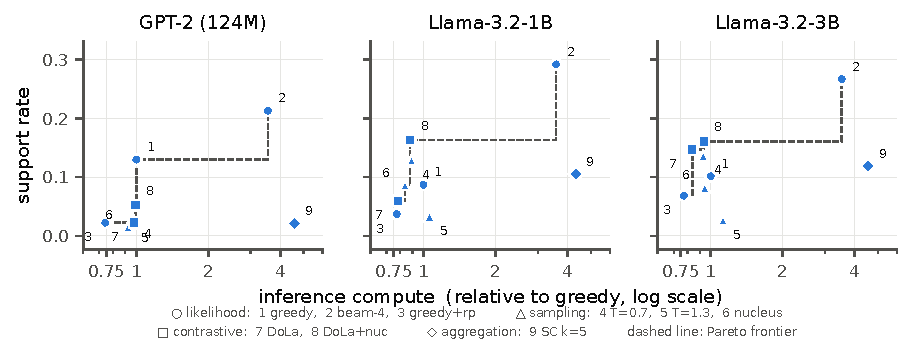
\includegraphics[width=\linewidth]{figures/f3_frontier.pdf}
  \caption{Support rate against inference compute relative to greedy, log
    scale. The dashed staircase marks the Pareto frontier. Self-consistency
    lies off the frontier at every scale.}
  \label{fig:frontier}
\end{figure*}

% T4 paired bootstrap, generated by scripts/table4.py
\begin{table}[t]
  \centering
  \small
  \begin{tabular}{l rrr}
    \toprule
    & \multicolumn{3}{c}{$\Delta$ support rate vs.\ nucleus-0.9} \\
    \cmidrule(lr){2-4}
    \textbf{Configuration} & \textbf{GPT-2} & \textbf{Llama-1B} & \textbf{Llama-3B} \\
    \midrule
    beam-4 & $+0.197^{*}$ & $+0.205^{*}$ & $+0.185^{*}$ \\
    greedy & $+0.115^{*}$ & $+0.000$ & $+0.019$ \\
    greedy+rp & $+0.007$ & $-0.050^{*}$ & $-0.014$ \\
    T=0.7 & $+0.013^{*}$ & $+0.042^{*}$ & $+0.055^{*}$ \\
    T=1.3 & $+0.005$ & $-0.054^{*}$ & $-0.055^{*}$ \\
    DoLa & $+0.007$ & $-0.027$ & $+0.065^{*}$ \\
    DoLa+nuc & $+0.037^{*}$ & $+0.076^{*}$ & $+0.079^{*}$ \\
    SC k=5 & $+0.005$ & $+0.019$ & $+0.037^{*}$ \\
    SC, one sample & $+0.004$ & $-0.010$ & $+0.008$ \\
    \bottomrule
  \end{tabular}
  \caption{Paired bootstrap over the 80 test prompts, 10{,}000 resamples, seeds averaged within a prompt. $^{*}$ marks a 95\% confidence interval excluding zero at the three decimals reported. DoLa's effect reverses sign with scale: negative at 1B, where the interval touches zero, and significantly better at 3B; the two intervals are disjoint. Self-consistency reaches significance only at 3B, where DoLa+nucleus delivers twice the gain at a fifth of the compute.}
  \label{tab:paired}
\end{table}


\section{Discussion}

\paragraph{What to use.} For a small open model where factual support matters
and inference compute is available, beam search is the answer, and the
diversity collapse must be accepted rather than mitigated --- the
repetition-penalty control shows that removing the repetition also removes most
of the factuality. Where compute is constrained, DoLa under nucleus sampling is
the best option at both Llama scales, delivering the largest significant gain
over nucleus of any configuration at no more than greedy's token cost.
Self-consistency is not worth its price at any scale we measured.

\paragraph{Why self-consistency fails here, stated as a claim others can use.}
Majority voting works when the output space has a mode that coincides with the
correct answer; for open-ended generation the mode is the model's most typical
continuation, which for an unfamiliar entity is often its most practised
fabrication. Agreement is therefore a weak signal rather than a misleading
one: the medoid beats the pool mean by $+0.028$ and $+0.029$ on the Llamas,
but that is only about a fifth of the distance to the oracle. The
decomposition locates the limit in the selector rather than the samples --- the
pool contains samples more than twice as good as the one it returns.

\section{Conclusion}

Holding the model, prompts, seeds and inference budget fixed while varying only
the decoder shows that the decoding choice is a factuality intervention of the
same order as a change in model scale, and that its cost is routinely
understated. Beam search buys factual support with diversity and compute;
DoLa's layer contrast helps wherever the sampler is matched and pays for it in
diversity; and aggregation by
self-consistency, extended to open-ended text, is dominated once compute is
priced in. Both halves of the tradeoff have to be measured at a matched budget
for any of these statements to be well defined.

\section*{Limitations}

\paragraph{Support is not truth, and coverage is unmeasured.} The metric asks
whether a claim is entailed by one Wikipedia page. A true claim the page omits
scores as unsupported, and we cannot say how often that happens: the human
label scheme was designed to need no world knowledge, which makes it objective
but merges ``true but absent from the page'' into ``not addressed''. This is
the largest open limitation of the measurement, and the stratum effect should
be read as memorisation and/or reference coverage, never as memorisation alone.

\paragraph{Measurement error, quantified but not removed.} Verifying sentences
rather than atomic facts forces an all-or-nothing call on mixed content: 23 of
100 human-labelled sentences mixed established and unestablished claims, so
absolute numbers are not comparable with published FActScore values. The
verifier is high-recall and low-precision; we report calibrated rates beside
raw ones, but the calibration rests on 100 labels and assumes a constant error
rate across configurations. Top-5 retrieval additionally loses roughly 3\% of
all sentences the page would support (Appendix~\ref{app:robustness}), and the
headline numbers are not corrected for it.

\paragraph{Scope of the claims.} Medoid selection is not majority voting: our
negative result concerns the extension we defined, and does not transfer to
self-consistency on tasks with a discrete answer. DoLa runs through a pinned
community implementation rather than the authors' own code. Two Llama sizes
plus GPT-2 is a trend, not a scaling law, and the 46 entities absent from the
pinned snapshot are table-heavy articles rather than a random sample, so the
pool is tilted away from the most heavily documented subjects. All models run
in \texttt{float16}, which the hardware forced.

\section*{AI Disclosure and Reflection}

An AI assistant (Claude Opus 5, Anthropic), used through the Claude desktop
application and Claude Code, supported a staged study plan, code review,
analysis and plotting scripts, and the drafting and revising of sections of
this paper. All code was executed and inspected by the authors, and every
number reported here was produced by running the committed scripts. The 100
manual validation labels in Section~4.5 were produced by the authors without AI
assistance: their purpose is to measure whether an automatic verifier agrees
with a human reader, and model-generated labels would have measured agreement
between two models.

Reflecting on the experience: design decisions changed under measurement rather
than under argument --- a bound on the evidence-pool artifact was withdrawn
once the human labels contradicted it, and the hypothesis that repetition
inflated beam search's score proved wrong in sign. The cost was a mid-stage
redesign of the label scheme.

\bibliography{custom}

\appendix
\section{Additional Results}

\subsection{Robustness of the ordering}
\label{app:robustness}

Collapsing repeated identical sentences before verification moves no
configuration by more than $0.026$, and moves them in the direction that would
favour the degenerate arms. Quadrupling retrieval depth to $m=20$ on the dev
entities raises support by $+0.022$ on average, with every one of 24
model--configuration cells moving in the same direction; beam-4 remains first
and $\tau=1.3$ last under both depths, while the middle ranks reorder among
configurations separated by less than their own intervals, which we therefore
report as a band rather than an ordering. An independent estimate from the
human labels puts retrieval failure at roughly 3\% of all sentences, agreeing
with the sweep.

% T3 verifier validation, generated by scripts/table3.py
\begin{table}[t]
  \centering
  \small
  \begin{tabular}{lr}
    \toprule
    \textbf{Quantity} & \textbf{Value} \\
    \midrule
    Labelled sentences & 100 \\
    \quad supported & 25 \\
    \quad contradicted & 7 \\
    \quad not addressed & 68 \\
    \midrule
    Sensitivity (TPR) & 0.947 \\
    False-positive rate & 0.041 \\
    Precision & 0.582 \\
    Balanced accuracy & 0.953 \\
    \midrule
    False positives & 36 \\
    \quad human-labelled \emph{not addressed} & 34 \\
    \quad human-labelled \emph{contradicted} & 2 \\
    False negatives & 1 \\
    \bottomrule
  \end{tabular}
  \caption{Verifier validation at $\theta=0.5$ against 100 blind human labels, stratified by entity stratum and entailment-probability band and reweighted to the full frame. The verifier is high-recall and low-precision: it almost never misses a supported sentence, but confidently entails claims the retrieved evidence does not address --- the neutral trap. Balanced accuracy peaks at $\theta=0.55$ (0.956) against 0.953 at $\theta=0.5$, so the pre-registered threshold is retained.}
  \label{tab:verifier}
\end{table}


\end{document}
